\vspace{0.5 cm}
\textcolor{blue} {\textit{Maël LE GALLIC}}
\vspace{0.3 cm}

In order to define the \emph{Bay of Biscay}, $\mathbb{G}$, we have to implement a SIVIA test that distinguish the earth from the sea. To deals with it, we realised a procedure which returns the sub-pavings of an input binary image. 
First of all, we compute the integral image of the binary image. The integral image (or summed area table) is a data structure which permit to quickly and efficiently generate the sum of pixel values in a rectangular subset of an image. The value at any pixel (i, j) in the integral image correspond to the sum of all the pixels above and to the left of (i, j). To compute the sum of pixel values of a rectangular subset of the image only four pixel values of the integral are required. Hence, the calculation time is constant and independent of the size of the rectangular area. This sum of v(i,j) over the rectangle spanned by A, B,C and D is:

$$\sum_{\begin{smallmatrix} i_A < i \le i_C \\ j_A < j \le j_C \end{smallmatrix}} v(i,j) = V(D) + V(A) - V(B) - V(C)$$

\begin{figure}[!h] 
\center
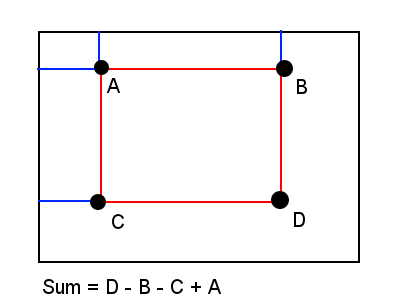
\includegraphics[scale=0.5]{integralImage.png} 
\caption{Description of computing a sum in an integral image } 
\label{fig: Integral image}
\end{figure}

Then, we use this integral image in our SIVIA test to say if the tested box is inside the 0-bit area, the 1-bit area or overlaps the two areas of the binary image. The procedure of this test is described below:

\begin{itemize}
\item We calculate the indexes of the four pixels corresponding to the vertices of the box.
\item We compute the number of pixel in the box: nbsPixel
\item By using the integal image, we compute the sum of pixel values in the box: sumPixel
\item We compare sumPixel with nbsPixel and 0 to classify the box.
\end{itemize}

\begin{algorithm}[H]
\caption{SIVIA Test ImageToBoxes}
\label{alg:one_boat_alg}
\begin{algorithmic}[1]
\REQUIRE $X$,$IntegralImage$\\
$i_A \leftarrow \textnormal{round(X[0].lb()/echellePixel) + i0}$\\
$j_A \leftarrow \textnormal{round(X[1].ub()/echellePixel) + j0}$\\
$i_C \leftarrow \textnormal{round(X[0].ub()/echellePixel) + i0}$\\
$j_C \leftarrow \textnormal{round(X[1].lb()/echellePixel) + j0}$\\
$ \textnormal{nbsPixel} \leftarrow (i_C - i_A) * (j_C - j_A)$\\
$ \textnormal{sumPixel} \leftarrow \textnormal{V(D) \ensuremath{+} V(A) \ensuremath{-} V(B) \ensuremath{-} V(C)}$
\IF {$\textnormal{sumPixel == 0}$}
\RETURN $\textnormal{OUT}$
\ELSIF {$\textnormal{sumPixel == nbsPixel}$}
\RETURN $\textnormal{IN}$
\ELSE
\RETURN $\textnormal{UNKNOWN}$
\ENDIF
\end{algorithmic}
\end{algorithm}

\vspace{1cm}
An example of the application of the SIVIA algorithm with the ImageToBoxes test is shown below. In input we have a binary image of the Biscay Bay and in output the resulting sub-pavings.
\begin{figure}[H]
\centering
    \begin{minipage}[b]{0.4\textwidth}
    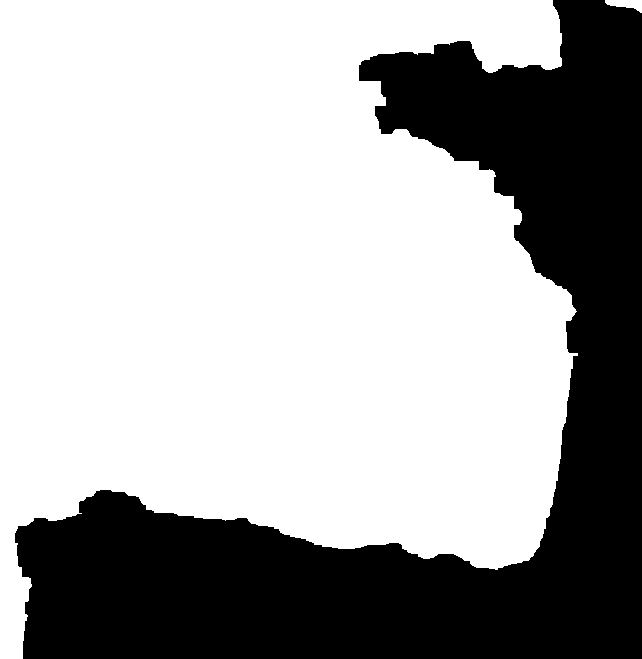
\includegraphics[scale=0.5]{Gascogne2.png}
	\caption{Binary image of the Biscay Bay } 
	\label{fig: Biscay Bay}
    \end{minipage}
    \begin{minipage}[b]{0.4\textwidth}
    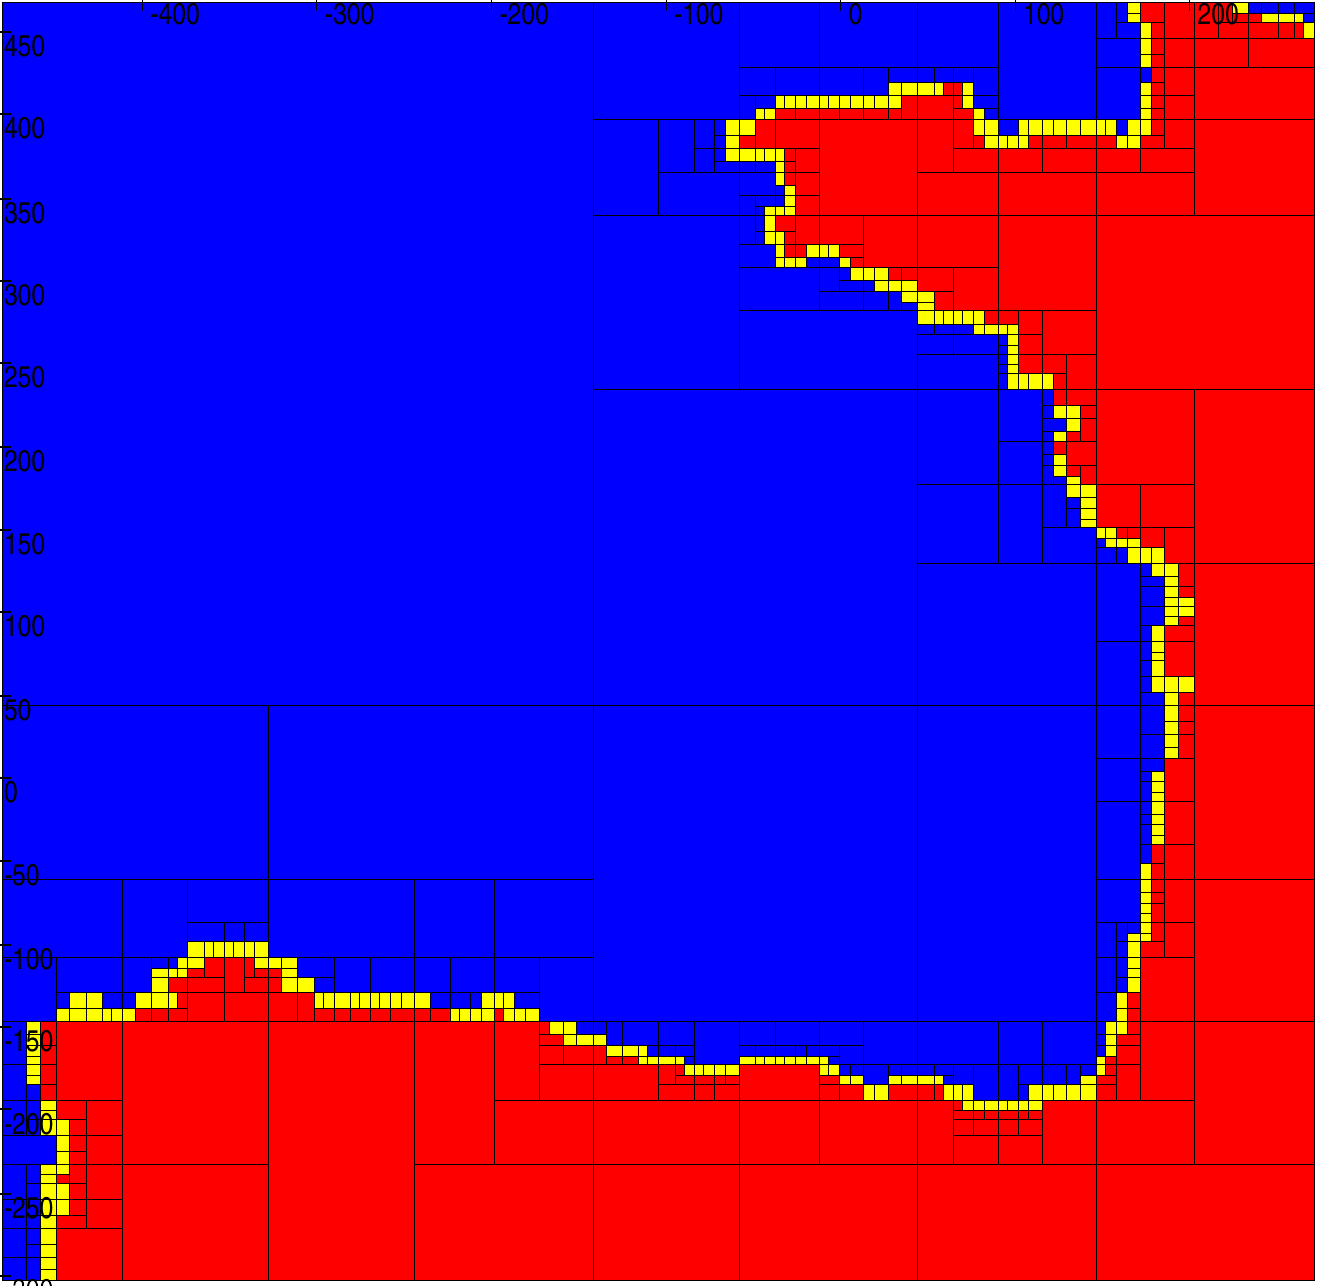
\includegraphics[scale=0.2]{GascogneBoxes.png} 
	\caption{Resulting sub-pavings of the Biscay Bay } 
	\label{fig: Sub-pavings of the Biscay Bay}
    \end{minipage}
\end{figure}

